\tikzset{every picture/.style={line width=0.75pt}} %set default line width to 0.75pt        

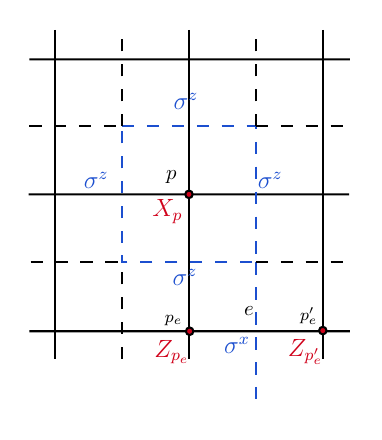
\begin{tikzpicture}[x=0.65pt,y=0.65pt,yscale=-1,xscale=1]
%uncomment if require: \path (0,300); %set diagram left start at 0, and has height of 300

%Straight Lines [id:da5739806697738756] 
\draw    (166.66,57.25) -- (166.66,240.08) ;
%Straight Lines [id:da7238586112220469] 
\draw    (255.74,148.67) -- (77.57,148.66) ;
%Shape: Rectangle [id:dp8929720889562809] 
\draw  [color={rgb, 255:red, 28; green, 79; blue, 207 }  ,draw opacity=1 ][dash pattern={on 4.5pt off 4.5pt}] (129.45,110.79) -- (203.86,110.79) -- (203.86,186.54) -- (129.45,186.54) -- cycle ;
%Straight Lines [id:da35697200962004727] 
\draw    (241.06,57.25) -- (241.06,240.08) ;
%Straight Lines [id:da3340888655283061] 
\draw    (92.25,57.25) -- (92.25,240.08) ;
%Straight Lines [id:da33148495583810944] 
\draw    (256.11,73.69) -- (77.94,73.67) ;
%Straight Lines [id:da6939189066147291] 
\draw    (256.11,224.8) -- (77.94,224.78) ;
%Shape: Ellipse [id:dp36619230768369126] 
\draw  [color={rgb, 255:red, 0; green, 0; blue, 0 }  ,draw opacity=1 ][fill={rgb, 255:red, 208; green, 2; blue, 27 }  ,fill opacity=1 ] (164.59,148.67) .. controls (164.59,147.5) and (165.51,146.56) .. (166.66,146.56) .. controls (167.8,146.56) and (168.72,147.5) .. (168.72,148.67) .. controls (168.72,149.83) and (167.8,150.77) .. (166.66,150.77) .. controls (165.51,150.77) and (164.59,149.83) .. (164.59,148.67) -- cycle ;
%Shape: Ellipse [id:dp9652736312822741] 
\draw  [fill={rgb, 255:red, 208; green, 2; blue, 27 }  ,fill opacity=1 ] (164.96,224.79) .. controls (164.96,223.63) and (165.89,222.68) .. (167.03,222.68) .. controls (168.17,222.68) and (169.1,223.63) .. (169.1,224.79) .. controls (169.1,225.95) and (168.17,226.9) .. (167.03,226.9) .. controls (165.89,226.9) and (164.96,225.95) .. (164.96,224.79) -- cycle ;
%Shape: Ellipse [id:dp10660430132854004] 
\draw  [fill={rgb, 255:red, 208; green, 2; blue, 27 }  ,fill opacity=1 ] (238.99,224.41) .. controls (238.99,223.25) and (239.92,222.31) .. (241.06,222.31) .. controls (242.2,222.31) and (243.13,223.25) .. (243.13,224.41) .. controls (243.13,225.57) and (242.2,226.52) .. (241.06,226.52) .. controls (239.92,226.52) and (238.99,225.57) .. (238.99,224.41) -- cycle ;
%Straight Lines [id:da37095650407934566] 
\draw [color={rgb, 255:red, 28; green, 79; blue, 207 }  ,draw opacity=1 ] [dash pattern={on 4.5pt off 4.5pt}]  (203.86,186.54) -- (203.86,268.75) ;
%Straight Lines [id:da6687270034078365] 
\draw [color={rgb, 255:red, 0; green, 0; blue, 0 }  ,draw opacity=1 ] [dash pattern={on 4.5pt off 4.5pt}]  (203.86,186.54) -- (257.8,186.54) ;
%Straight Lines [id:da8280996691564566] 
\draw [color={rgb, 255:red, 0; green, 0; blue, 0 }  ,draw opacity=1 ] [dash pattern={on 4.5pt off 4.5pt}]  (203.86,110.79) -- (257,110.79) ;
%Straight Lines [id:da8863115042170602] 
\draw [color={rgb, 255:red, 0; green, 0; blue, 0 }  ,draw opacity=1 ] [dash pattern={on 4.5pt off 4.5pt}]  (203.86,110.79) -- (203.86,57.8) ;
%Straight Lines [id:da5214859423647604] 
\draw [color={rgb, 255:red, 0; green, 0; blue, 0 }  ,draw opacity=1 ] [dash pattern={on 4.5pt off 4.5pt}]  (78.6,186.54) -- (129.45,186.54) ;
%Straight Lines [id:da3470737481060351] 
\draw [color={rgb, 255:red, 0; green, 0; blue, 0 }  ,draw opacity=1 ] [dash pattern={on 4.5pt off 4.5pt}]  (77.8,110.79) -- (129.45,110.79) ;
%Straight Lines [id:da692387720624561] 
\draw [color={rgb, 255:red, 0; green, 0; blue, 0 }  ,draw opacity=1 ] [dash pattern={on 4.5pt off 4.5pt}]  (129.45,110.79) -- (129.45,56.6) ;
%Straight Lines [id:da9061624023045722] 
\draw [color={rgb, 255:red, 0; green, 0; blue, 0 }  ,draw opacity=1 ] [dash pattern={on 4.5pt off 4.5pt}]  (129.45,240.2) -- (129.45,186.54) ;

% Text Node
\draw (145.06,150.32) node [anchor=north west][inner sep=0.75pt]  [font=\large,color={rgb, 255:red, 208; green, 2; blue, 27 }  ,opacity=1 ,xscale=0.75,yscale=0.75]  {$X_{p}$};
% Text Node
\draw (156.81,91.11) node [anchor=north west][inner sep=0.75pt]  [font=\large,color={rgb, 255:red, 28; green, 79; blue, 207 }  ,opacity=1 ,xscale=0.75,yscale=0.75]  {$\sigma ^{z}$};
% Text Node
\draw (106.97,135.11) node [anchor=north west][inner sep=0.75pt]  [font=\large,color={rgb, 255:red, 28; green, 79; blue, 207 }  ,opacity=1 ,xscale=0.75,yscale=0.75]  {$\sigma ^{z}$};
% Text Node
\draw (203.72,135.27) node [anchor=north west][inner sep=0.75pt]  [font=\large,color={rgb, 255:red, 28; green, 79; blue, 207 }  ,opacity=1 ,xscale=0.75,yscale=0.75]  {$\sigma ^{z}$};
% Text Node
\draw (156.31,188.94) node [anchor=north west][inner sep=0.75pt]  [font=\large,color={rgb, 255:red, 28; green, 79; blue, 207 }  ,opacity=1 ,xscale=0.75,yscale=0.75]  {$\sigma ^{z}$};
% Text Node
\draw (151.97,214.48) node [anchor=north west][inner sep=0.75pt]  [font=\footnotesize,xscale=0.75,yscale=0.75]  {$p_{e }$};
% Text Node
\draw (227.14,210.23) node [anchor=north west][inner sep=0.75pt]  [font=\footnotesize,xscale=0.75,yscale=0.75]  {$p'_{e }$};
% Text Node
\draw (146.14,228.46) node [anchor=north west][inner sep=0.75pt]  [font=\large,color={rgb, 255:red, 208; green, 2; blue, 27 }  ,opacity=1 ,xscale=0.75,yscale=0.75]  {$Z_{p_{e }}$};
% Text Node
\draw (220.39,228.19) node [anchor=north west][inner sep=0.75pt]  [font=\large,color={rgb, 255:red, 208; green, 2; blue, 27 }  ,opacity=1 ,xscale=0.75,yscale=0.75]  {$Z_{p'_{e }}$};
% Text Node
\draw (184.86,226.94) node [anchor=north west][inner sep=0.75pt]  [font=\large,color={rgb, 255:red, 28; green, 79; blue, 207 }  ,opacity=1 ,xscale=0.75,yscale=0.75]  {$\sigma ^{x}$};
% Text Node
\draw (152.67,134.4) node [anchor=north west][inner sep=0.75pt]  [xscale=0.75,yscale=0.75]  {$p$};
% Text Node
\draw (196,209.73) node [anchor=north west][inner sep=0.75pt]  [xscale=0.75,yscale=0.75]  {$e $};


\end{tikzpicture}
